\chapter{Records and Single-Segment Persistence}
This chapter answers a basic but important question: after a message is written to a file, how can we know that it is complete, in order, and recoverable after a process restart? Conceptually, a Kafka partition is an append-only log. This course first encodes each record directly into a single-segment file, then adds segmentation, indexing, and retention. An offset is a logical position and cannot be replaced with a file byte position.

\begin{figure}[ht]
\centering
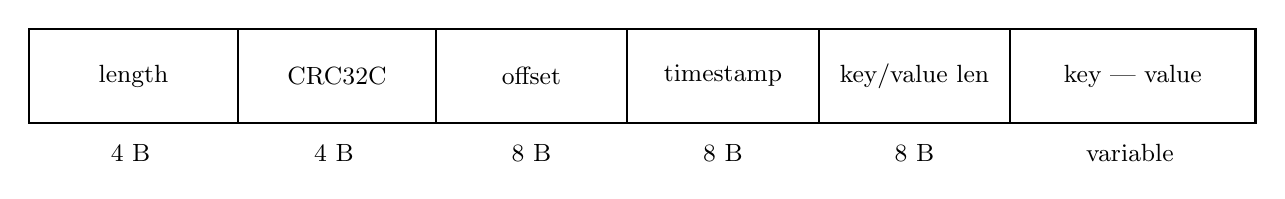
\begin{tikzpicture}[x=0.76mm,y=1mm,font=\small]
\draw[thick] (0,0) rectangle (35,12); \node at (17.5,6) {length};
\draw[thick] (35,0) rectangle (68,12); \node at (51.5,6) {CRC32C};
\draw[thick] (68,0) rectangle (100,12); \node at (84,6) {offset};
\draw[thick] (100,0) rectangle (132,12); \node at (116,6) {timestamp};
\draw[thick] (132,0) rectangle (164,12); \node at (148,6) {key/value len};
\draw[thick] (164,0) rectangle (205,12); \node at (184.5,6) {key | value};
\node[below=4pt] at (17,0) {4 B}; \node[below=4pt] at (51,0) {4 B};
\node[below=4pt] at (84,0) {8 B}; \node[below=4pt] at (116,0) {8 B};
\node[below=4pt] at (148,0) {8 B}; \node[below=4pt] at (184,0) {variable};
\end{tikzpicture}
\caption{A disk record. length does not include its own leading 4 bytes.}
\end{figure}

\lessonsection{1}{Record Encoding and Decoding}
\goals{Define stable on-disk boundaries so writers and readers assign the same meaning to the bytes.}{Understand signed lengths, fixed-width integers, UTF-8 bytes, and CRC32C; prior knowledge of file scanning is not required.}
\background{The format is big-endian: \pathcode{length:int32 | crc32c:int32 | offset:int64 | timestamp:int64 | keyLength:int32 | valueLength:int32 | key | value}. length is counted from the CRC field and has a legal range of 28 to 1,048,576; keyLength=-1 means null, while 0 means an empty key. value must be present but may have length 0. CRC32C covers bytes from the beginning of offset through the end of value; neither the length prefix nor the CRC field itself participates in the check. Both offset and timestamp must be nonnegative. Validate the length before consuming bytes according to the declared fields so that a malicious or corrupt length can be distinguished from a genuinely short buffer. Decoding consumes exactly one record; even if another record follows, it must not consume the suffix.}
\providededit{The \pathcode{LogRecord}, \pathcode{RecordData}, \pathcode{CourseException}, and \pathcode{ErrorCode} types, big-endian fields, and CRC32C utility types are provided. Array ownership is delegated to the data types; do not make duplicate copies for every field access.}{\pathcode{exercises/src/main/java/io/simplekafka/storage/RecordCodec.java}: \method{encode(LogRecord)}, \method{decode(ByteBuffer)}.}
\lessoncontract{Encoding must allocate exactly the required record space; a record's offset and timestamp cannot be negative, and value cannot be null. Insufficient input for decoding is \method{INVALID_REQUEST}; a format error or CRC mismatch is \method{CORRUPT_RECORD}. On success, the buffer position is exactly after this record, leaving subsequent bytes untouched for the next decode. A null key must not be confused with an empty key.}
\lessonhints{Split the format table into a “fixed-width header” and a “variable-length tail,” and list the byte count of each field first.}{Make the CRC's protected start and end boundaries explicit; the definition of length is not the same as the total number of allocated bytes.}{Write round-trip and single-byte corruption tests, then separately observe which protocol error should result from a short buffer, an illegal length, and a failed checksum.}
\expected{Encode and then decode a record with offset 7, a null key, timestamp 9, and value bytes equal to the UTF-8 encoding of “值”. The offset, key, timestamp, and bytes must be preserved. Flipping one bit in value makes decode report \method{CORRUPT_RECORD}; a buffer shorter than one complete record reports \method{INVALID_REQUEST}. These cases correspond to \method{Step01Test} and also verify that decoding does not consume a record immediately following this one.}
\pitfalls{Counting the length prefix in length, including the CRC field in its own CRC, or interpreting a null key as an empty array all break interoperability. CRC detects corruption; it is not a security signature. Real Kafka usually organizes records into batches and has richer compression and batch formats. This course deliberately uses a single-record format so field boundaries are visible; it does not claim that this is Kafka's disk format.}
\lessoncommand{1}
\lessonquestions{Why can't a record's logical offset be inferred from its file byte position?}{What can a successful CRC check prove, and what can it not prove?}

\lessonsection{2}{Log Append}
\goals{Implement continuous offset allocation and observable persistence for a single-segment log.}{Know the encoding from Step 1 and distinguish locking, full-write loops, and writes at file positions.}
\background{Appending turns data in memory into ordered log facts. The partition's local lock serializes appends to the same partition so competing batches do not receive interleaved or overlapping offsets. A single ordinary FileChannel.write may write only part of a buffer, so the provided \method{ChannelIO.writeFully} must be used. After writing a batch, call \method{force(false)} before publishing the append result; \method{AppendResult(firstOffset,nextOffset)} uses a half-open interval, for example [0,3) for three records. If an I/O error occurs during writing, the course does not guarantee atomic rollback of the whole batch; recovery after restart is responsible for identifying a physical tail fragment.}
\providededit{The \method{SegmentLog} path, FileChannel, lock, baseOffset, nextOffset, and \method{close()} are given; record encoding and partial-write I/O can be reused.}{\pathcode{exercises/src/main/java/io/simplekafka/storage/SegmentLog.java}: \method{append(List<RecordData>)}.}
\lessoncontract{An empty batch reports \method{INVALID_REQUEST}. A nonempty batch receives continuous offsets starting at the current LEO while holding the lock; precheck all parameters and each record's size before writing the batch so known-invalid input cannot write a prefix and then fail. After all records have been written and force succeeds, return the first offset and the next offset. The established types and codec contract constrain each record's timestamp and data validity.}
\lessonhints{Express the result using the first and next offsets of a batch; do not mistake “record count” for the first offset of the next batch.}{Think about which errors can be detected before acquiring the lock and which state must be read while holding it.}{Have concurrent appends compete on the same log instance and observe batch-level ordering and file contents; do not assert only the final LEO.}
\expected{Append three records and then two records to an empty segment; the expected results are [0,3) and [3,5), respectively, and decoding the file yields offsets 0, 1, 2, 3, and 4. The result intervals for two concurrent batches of two records must not overlap, and the total record count must be four. These are the actual-file and concurrency checks in \method{Step02Test}.}
\pitfalls{Writing first and discovering that a record is too large later leaves an invalid partial batch. Updating nextOffset without forcing or checking the write is also wrong. Real Kafka uses batching, background I/O, and more complex persistence policies; this course explicitly forces after every append so the boundary is observable, not to model Kafka's performance policy of synchronously writing every message to disk.}
\lessoncommand{2}
\lessonquestions{Why should the entire batch be validated before any disk write?}{What does a successful force mean, and what does it not mean?}

\lessonsection{3}{Offset-Based Reads}
\goals{Read complete records from a specified offset while honoring both record-count and byte budgets.}{Distinguish offsets, in-segment byte positions, record integrity, and cursor state.}
\background{Consumers request logical offsets, while file reads require physical byte positions. The first version of the public read starts at the beginning of the segment; the index in the next chapter will provide the log with a physical-position hint near a logical offset. A hint can shorten the search but cannot change offset semantics. Each record is an indivisible return unit: if the next complete record does not fit the budget, do not return part of it. The budget includes the length prefix. Explicit-position FileChannel reads avoid sharing a mutable channel cursor between reads and appends.}
\providededit{Segment lifecycle management and record decoding are complete; the public \method{read(offset,maxRecords,maxBytes)} passes a default hint to the internal method.}{\pathcode{exercises/src/main/java/io/simplekafka/storage/SegmentLog.java}: \method{readFrom(long offset,long bytePositionHint,int maxRecords,int maxBytes)}.}
\lessoncontract{offset may range from baseOffset through LEO (reading at LEO returns empty); an offset outside the segment's valid range reports \method{OFFSET_OUT_OF_RANGE}. maxRecords and maxBytes must be positive. Return records with continuous offsets that do not exceed either budget; if the first record alone exceeds the byte budget, return an empty result. A valid hint must be at a record boundary and cannot pass the target offset, or report \method{INVALID_REQUEST}. Reads must not move the append position or change LEO.}
\lessonhints{Treat “find a candidate byte position” and “which offset should the output start at?” as two separate questions.}{For the byte budget, calculate the size of each complete record, including the length prefix; do not approximate it using payload bytes.}{Design one hint that points to a boundary before the target and another that points past the target, then verify the conditions for accepting and rejecting them.}
\expected{After appending offsets 0–4, \pathcode{read(2, 2, 4096)} returns offsets 2 and 3. Then call \pathcode{readFrom(2,hint,2,4096)} with hint set to the actual starting byte position of the offset 1 record in the file; it should still return offsets 2 and 3. The hint is a physical position, not the numeric logical offset. \pathcode{read(5, 2, 4096)} returns empty. Reading from offset 1 with a 66 byte budget returns exactly 1 and 2; a smaller budget returns only 1. If the first complete record exceeds maxBytes, return empty rather than partial bytes. These cases correspond to \method{Step03Test}.}
\pitfalls{Offset 2 is not file byte 2; confusing them will randomly drop records once an index is introduced. Ignoring the prefix in the budget exceeds the caller's memory budget. A real Kafka fetch usually negotiates batch and network-byte limits; this implementation returns one record atomically, and the next chapter handles the total budget across segments.}
\lessoncommand{3}
\lessonquestions{Why can a sparse index provide only a search starting point, not directly determine the read result?}{What problem would returning a partial record cause when the first record is larger than maxBytes?}

\lessonsection{4}{Crash Recovery}
\goals{Recover a continuous LEO from a log that may have closed partway through a write, and repair only cases that can be proven to be an incomplete tail.}{Understand record boundaries, physical truncation, and error categories.}
\background{A crash can occur while writing the length prefix, fixed header, or payload. If EOF falls inside the last record's header or body, data before the last complete record can still form a valid log, so the file can be truncated to the preceding record boundary. However, a complete record with a bad CRC, an illegal length, or a discontinuous offset is not something that can be “safely discarded as a tail.” Silently truncating complete but damaged evidence would report a media failure as successful recovery. Recovery starts with the expected offset set to baseOffset, scans to the last valid boundary, and returns the next writable position.}
\providededit{\method{SegmentLog.open(file,baseOffset)} opens an existing file and invokes recovery; the codec from Step 1 and file layout from Steps 2 and 3 are established.}{\pathcode{exercises/src/main/java/io/simplekafka/storage/SegmentLog.java}: \method{recover()}.}
\lessoncontract{On success, return the recovered LEO so the next append continues from it; only an incomplete record at the end of the file may be truncated. A complete record with a bad CRC, illegal length, or discontinuous offset must fail with \method{CORRUPT_RECORD}; do not skip the bad record and continue scanning. Underlying I/O exceptions use \method{STORAGE_ERROR} and preserve the cause.}
\lessonhints{First define the “shared state” after each successful scan: the current valid byte boundary and the next expected offset.}{Classify EOF with too few bytes separately from a fully read record whose contents are incorrect.}{Construct two reopen tests: one with a partial tail record and one with a complete record whose CRC is corrupt. Confirm that only the former changes the file length.}
\expected{The file contains complete offsets 0 and 1, followed by a partial body for offset 2. After reopening, LEO=2 and the file is truncated exactly to the end of the second record; appending one record gives offset 2. If offset 1 is complete but its CRC is wrong, reopen must fail rather than treating it as a tail fragment. These cases correspond to \method{Step04Test}.}
\pitfalls{“Truncate whenever scanning reports an error” swallows corruption and format errors in complete records; “any EOF makes the file invalid” cannot handle a normal crash tail. \method{force(false)} expresses this course's write intent; it is not proof of power-loss safety. Real Kafka also has segment recovery, index repair, log validation, and more complex cleanup policies; this step recovers only the boundary of one segment.}
\lessoncommand{4}
\lessonquestions{Which byte-level evidence is enough to identify an incomplete tail, and which evidence must be reported as corruption?}{Why should recovery return LEO rather than the offset of the last record?}
